\documentclass[notes, dvipsnames]{beamer}

\usepackage{default}
\usepackage[dutch]{babel}
\usepackage{pgfpages}
\usepackage{pgf-pie}
\usepackage{ifthen}
\usepackage{qtree}
\usepackage[utf8]{inputenc}

\usetheme{Frankfurt}
\usecolortheme{beaver}
\setbeamertemplate{note page}{\pagecolor{yellow!25}\insertnote}
%\setbeamertemplate{note page}{\pagecolor{white}\insertnote}

\title{Automatisch vertalen van logigrammen naar een getypeerde logica}
\subtitle{Thesisverdediging}

\author{Jens Claes}
\date{28 juni 2017}

\newcommand{\seperation}{
	\vspace{1em}
	\ppause
}
\newcommand{\sseperation}{
	\vspace{1em}
}
\newcommand{\hitem}{
	\ppause
	\item
}
\newcommand{\ppause}{\onslide<+>}
\newcommand{\nnote}[1]{\note<.>{#1}}
\setbeamercovered{%
	still covered={\opaqueness<1->{0}},
	again covered={\opaqueness<1->{60}}
}
%\setbeameroption{hide notes} % Only slides
\setbeameroption{show notes on second screen=right} % Both

\newcommand{\attention}[1]{\textcolor{ForestGreen}{#1}}

%\graphicspath{ {../images/} }

\setbeamertemplate{bibliography item}{\insertbiblabel}
\AtBeginSection[]
{
   \begin{frame}
        \frametitle{Inhoudstafel}
        \tableofcontents[ 
              currentsection,
              hideothersubsections
            ] 
   \end{frame}
}
\begin{document}
	\frame{\titlepage}

  \begin{frame}
    \frametitle{Inhoudstafel}
    \tableofcontents[hidesubsections] 
  \end{frame}

  \section{Inleiding}
	\begin{frame}{Knowledge Base Systems}
		\begin{itemize}
      \hitem Invoer: Kennisbank
      \item Specificatie van de wereld

			\seperation
      \item Inferenties \cite{idp}
        \begin{itemize}
          \hitem Propagatie
          \hitem Model expansie
          \hitem Bevraging
        \end{itemize}

      \seperation
      \item Kennisrepresentatietaal
      \nnote{
        Moeilijk om te lezen, schrijven en leren
      }
		\end{itemize}
	\end{frame}

	\begin{frame}{Controlled Natural Language (CNL)}
		\begin{itemize}
      \hitem Gecontroleerde natuurlijke taal
      \item Subset natuurlijke taal

      \seperation
      \item Makkelijker te schrijven/lezen
      \hitem Formele semantiek
      \nnote{Slecht gedocumenteerd}
		\end{itemize}
	\end{frame}

	\section{Probleem}
	\begin{frame}{Probleemstelling}
		\begin{itemize}
      \hitem Formele taal
        \begin{itemize}
          \hitem Toegankelijk
          \item Rijk genoeg
          \item Toepasbaar binnen KBS
          \nnote{CNL?}
        \end{itemize}

      \seperation
      \item Extra: types

      \seperation
      \item Logigrammen (uit \cite{logigrammen})
        \nnote{Als eerste test. Zeker nog niet rijk genoeg maar ``toegankelijk'' en ``toepasbaar binnen KBS'' wel al te testen}
		\end{itemize}
	\end{frame}

	\begin{frame}{Logigrammen}
    \begin{figure}
      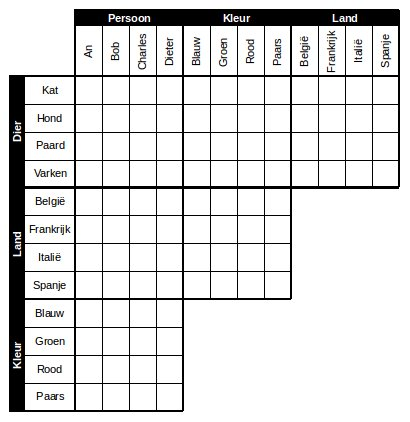
\includegraphics[width=0.6\textwidth]{logigram.jpg}
    \end{figure}
    \note{
      \begin{itemize}
        \item Aantal domeinen (nationaliteiten, dieren, kleuren, ...)
        \item Aantal domeinelementen (Noor, Brit, kat, hond, ...)
        \item 1 bijectie tussen elk paar domeinen
        \item Aantal hints/clues: constraints op die bijecties
        \item Doel: Zoek de waarde van de bijecties

        \sseperation

        \item Hints in natuurlijke taal
        \item Redelijke uniforme zinstructuur

        \sseperation

        \item Geschikt om automatisch om te zetten naar logica
      \end{itemize}
    }
	\end{frame}

	\begin{frame}{Inferenties op logigrammen}
		\begin{itemize}
      \hitem Oplossen
      \hitem Status clues
      \hitem Hint
      \hitem Schrijfhulp
		\end{itemize}
	\end{frame}
	
	\section{Systeem}
  % \subsection{Overzicht}
	\begin{frame}{Systeem Thesis}
		\begin{enumerate}
      \hitem Vertaal + leid types af
      \nnote{Invoer: lexicon + clues, dat is alles!}
      \hitem Infereer domeinen
      \nnote{Interactie met gebruiker mogelijk}
      \hitem Formeel vocabularium
      \hitem Axioma's
      \hitem Pas inferentie toe
      \nnote{Wij beperkt tot ``oplossen'' maar we hebben volledige specificatie}
		\end{enumerate}
	\end{frame}

  % \subsection{Framework}
	\begin{frame}{Framework}
		\begin{itemize}
      \hitem Blackburn en Bos \cite{Blackburn2005, Blackburn2006}
      \nnote{Goed gedocumenteerd}

      \seperation
      \item Compositioneel
      \item $\lambda$-calculus
      \item Semantiek in lexicon
      \nnote{
        Betekenis van de woorden (lambda-formules) naar boven toe propageren
      }
      \hitem 4 onderdelen
      \nnote{
        4 onderdelen staan los van elkaar
        \begin{itemize}
          \item Lexicon/Vocabularium: per probleem, taalkundige categorieën
          \item Grammatica: contextvrij, categorial combinatorial grammar (Baral et al. \cite{Baral2008}), ...
          \item Lexicale semantiek: eerste-orde logica, discourse representation structures, event-based logic, ...
          \item Grammaticale semantiek: licht gekoppeld aan grammatica en lexicale semantiek
        \end{itemize}
      }

      \seperation
      \item Aangepast voor logigrammen
      \nnote{
        \begin{itemize}
          \item Lexicon: enkel existentiële kwantificatie
          \item PN: valsspelen
          \item werkwoorden en voorzetsels: predicaten
          \item Algemene en specifieke grammaticale regels
          \item Alldifferent, simpele arithmetiek
          \item Toevoegen types
        \end{itemize}
      }
		\end{itemize}
	\end{frame}

  % \subsection{Types}
	\begin{frame}{Types}
    \begin{itemize}
      \hitem Het huis drinkt de tuin

      \seperation
      \item Via taalkundige ``features''
      \nnote{
        Bv. $NP[num]$ meervoud of enkelvoud
      }

      \seperation
      \item Simpel typesysteem
      \nnote{
        \item basistypes + pair-types voor werkwoorden en voorzetsels
        \item $NP[type]$: één van de domeinen
        \item $TV[type]$: bijectie tussen twee domeinen
      }
    \end{itemize}
	\end{frame}

  \begin{frame}{Inferentie Domeinen}
    \begin{itemize}
      \hitem Type-inferentie
      \nnote{Lexicon geen type-informatie}
      \hitem Type uniek per woord
      \nnote{Opdeling van woorden in domeinen}
      \hitem Taalkundige vragen gebruiker
      \nnote{Synoniemen, mogelijk lijdend voorwerp, 2 woorden zelfde type?}
    \end{itemize}
  \end{frame}

  \begin{frame}{Een complete specificatie}
    \begin{itemize}
      \hitem Formeel vocabularium
      \nnote{
        \item Afgeleid uit types
        \item Domeinen = Constructed Type (DCA, UNA)
        \item Getallen = Subsets
        \item Andere types ``John follows the tour with 54 people'' ook constructed types
      }
      \hitem Axioma's
      \begin{itemize}
        \hitem Bijectie
        \hitem Symmetriebrekers
        \hitem Synoniemen
        \hitem Equivalentierelatie (transitief, symmetrisch)
      \end{itemize}
    \end{itemize}
  \end{frame}

  \section{Evaluatie}
  \begin{frame}{Evaluatie}
    \begin{itemize}
      \hitem Puzzle Baron's Logic Puzzles Volume 3 \cite{logigrammen}
      \nnote{
        \item Training = eerste 10
        \item Test = volgende 10
      }

      \seperation
      \item Kleine aanpassingen
      \item Automatisch oplosbaar
    \end{itemize}
  \end{frame}

  \begin{frame}{Evaluatie}
    \begin{table}[t]
      \centering
      \begin{tabular}{lc}
        \hline
        \textbf{Probleem} & \textbf{Aantal voorkomens} \\ 
        \hline
        ``the one'' & 15 \\
        Ongezien gebruik koppelwerkwoord & 6 \\
        Slecht gestructureerde bijzin & 6 \\
        Passieve zin & 1 \\
        Bezittelijk voornaamwoord & 1 \\
        Slecht gestructureerde naamwoordgroep & 1 \\
        \hline
        Gehele getallen & 3 \\
        Superlatief & 1 \\
        ``Of the two ...'' & 1 \\
        \hline
        Slecht getypeerd werkwoord & 14 \\
        Slecht getypeerde naamwoordgroep & 5 \\
        \hline
        Meer dan één woordvorm eigennaam  & 1 \\
        \hline
        Overbodig woord & 7 \\
        Ontbrekend woord (ellips) & 3 \\
        \hline
      \end{tabular}
      \caption{Een overzicht van de aanpassingen}
      \label{tbl:resultaten}
    \end{table}
  \end{frame}

  \section{Conclusie}
  \begin{frame}{Conclusie}
    \begin{itemize}
      \hitem Goed framework
      \nnote{ Voor CNL met formele semantiek}
      \hitem Inferentie op CNL
      \nnote{ Enkel ``oplossen'' uitgewerkt maar specificatie is er dus de rest kan ook }
      \hitem Getypeerde CNL
      \nnote{ Nu type-inferentie + getypeerde logica, meer is mogelijk, ook moeilijker type-systeem
      \item e.g. to order food or drinks (multiple types per woord)}
    \end{itemize}
  \end{frame}

			
	\section{Referenties}
	\begin{frame}[allowframebreaks]{Referenties}
		\bibliographystyle{plain}
		\bibliography{../thesis/referenties}
	\end{frame}
	
\end{document}
